\documentclass{article}
\usepackage[english,russian]{babel}
\usepackage{textcomp}
\usepackage{geometry}
  \geometry{left=2cm}
  \geometry{right=1.5cm}
  \geometry{top=1.5cm}
  \geometry{bottom=2cm}
\usepackage{tikz}
\usepackage{multicol}
\usepackage{hyperref}
\usepackage{amsmath}
\usepackage{listings}
\pagenumbering{gobble}

\lstset{
  language=C,
  basicstyle=\linespread{1.1}\ttfamily,
  columns=fixed,
  basewidth=0.5em,
  keywordstyle=\color{blue}\bfseries,
  commentstyle=\color{gray},
  stringstyle=\ttfamily\color{orange!50!black},
  showstringspaces=false,
  backgroundcolor=\color{white},
  breaklines=true,
  breakatwhitespace=true,
  xleftmargin=5mm,
  keepspaces = true,
  extendedchars=\true,
  tabsize=4,
  upquote=true,
}

\lstdefinestyle{csMiptBash}{
breaklines=true,
frame=tb,
language=bash,
breakatwhitespace=true,
alsoletter={*()"'0123456789.},
alsoother={\{\=\}},
basicstyle={\ttfamily},
keywordstyle={\bfseries},
literate={{=}{{{=}}}1},
prebreak={\textbackslash},
sensitive=true,
stepnumber=1,
tabsize=4,
morekeywords={echo, function},
otherkeywords={-, \{, \}},
literate={\$\{}{{{{\bfseries{}\$\{}}}}2,
upquote=true,
frame=none
}


\begin{document}
\title{Установка необходимых программ в ОС Windows. \vspace{-5ex}}\date{}\maketitle
\section*{Справка по различным компиляторам}
Основные программы, которыми мы будем пользоваться -- это компиляторы для языков C и C++. Компилятор -- это программа, которая переводит код на языке программирования в набор машинных команд (исполняемый файл). Существует множество различных компиляторов для языков C и C++. Разберём самые популярные из них.

\begin{enumerate}
\item \textbf{GCC} -- это свободный набор компиляторов. Работает на Unix-подобных системах (то есть в Linux, macOS и других). Де-факто является стандартом в этих системах. На данный момент является самым популярным компилятором C и C++ в мире. 
\item \textbf{Clang} -- разработан как альтернатива GCC с акцентом на скорость компиляции и понятные сообщения об ошибках. Работает как на Windows, так и на Unix-подобных системах.
\item \textbf{MSVC} -- это компилятор C/C++ от Microsoft, который является частью Visual Studio. Широко используется в корпоративной среде и для разработки Windows-приложений. Работает только на Windows.
\item \textbf{MinGW} -- порт компилятора GCC для Windows. Старается быть похожим на GCC насколько это возможно.
\end{enumerate}
В данном курсе мы будем использовать компилятор MinGW. Важно отметить, что, так как MinGW -- это порт GCC, то в командной строке для его вызова также используется исполняемый файл \texttt{gcc}.


\section*{Установка пакетного менеджера MSYS2}
MSYS2 -- это среда разработки и пакетный менеджер для Windows, который упрощает установку программ и библиотек. Без неё пришлось бы всё устанавливать вручную, что гораздо сложнее и занимает больше времени.

Для установки MSYS2 перейдите на сайт \href{https://www.msys2.org/}{www.msys2.org} и скачайте установщик. Для обычного ноутбука с 64-битной версией Windows установщик будет называться так: \texttt{msys2-x86-64-дата\_сборки.exe}, где дата сборки будет представлена восемью цифрами. Установите MSYS2 на компьютер. Желательно устанавливать в путь по умолчанию, то есть в \texttt{C:\textbackslash msys64}. Если устанавливаете в другом месте, убедитесь, что путь не содержит содержит пробелов, кириллицы и других странных символов.

После установки откройте меню Пуск и начните вводить \textit{"MSYS2"}. Появится несколько приложений, которые можно открыть. Различные приложения -- это разные виды окружений, поддерживаемые MSYS2. В данном курсе мы будем использовать окружение UCRT64, так как оно более современное. Откройте приложение \texttt{MSYS2 UCRT64}.
В результате вы должны увидеть следующее окно:

\begin{center}
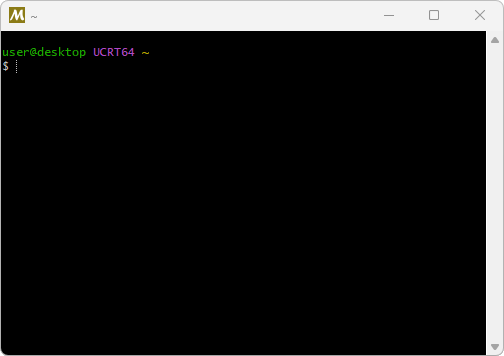
\includegraphics[scale=0.6]{../images/install-4-terminal.png}
\end{center}

В этом окне вы можете как устанавливать программы, компилировать свои программы и делать всё, что можно в обычном терминале. Данный терминал поддерживает такой же синтаксис, что терминал Linux.

\section*{Установка программ с помощью MSYS2}
Для установки программ MSYS2 использует пакетный менеджер \texttt{pacman}, изначально разработанный для Linux. Вот некоторые команды данного пакетного менеджера:\\

\texttt{
\begin{tabular}{ l | l }
 pacman -Ss строка          & найти в интернет-репозиториях пакеты, названия которых содержат данную строку \\
 pacman -Qs строка       	& среди уже установленных, найти пакеты, названия которых содержат данную строку \\
 pacman -S пакет           	& установить пакет и его зависимости \\ 
 pacman -Rs пакет          	& удалить пакет и его зависимости, которые больше никому не нужны \\ 
 pacman -Q           		& показать список всех установленных пакетов \\ 
 pacman -Syu           		& обновить все пакеты \\ 
\end{tabular}
}

\noindent Для того, чтобы узнать имя пакет можно использовать команду \texttt{pacman -Ss} или просто загуглить это название. Например, если вы хотите установить \texttt{gcc}, то просто загуглите \textit{"msys2 install ucrt64 gcc"}. После этого находите первую ссылку на сайт \texttt{msys2.org}, скорей всего эта ссылка будет на нужный вам пакет. В данном случае важно использовать поисковик Google, так как он лучше ищет всё, что связано с программированием.

Сейчас нам нужно установить только компилятор MinGW, базовые программы coreutils и систему контроля версий git, но в дальнейшем нам могут понадобиться другие программы и библиотеки.

\subsection*{Обновление пакетов}
Для обновления всех уже установленных пакетов запустите команду:
\begin{lstlisting}[style=csMiptBash]
$ pacman -Syu
\end{lstlisting}
Следует запустить эту команду при первом запуске для обновления установленных по умолчанию пакетов.

\subsection*{Установка компилятора MinGW (gcc для Windows)}
Для установки компилятора MinGW просто напишите в MSYS2 терминал:
\begin{lstlisting}[style=csMiptBash]
$ pacman -S mingw-w64-ucrt-x86_64-gcc
\end{lstlisting}

\subsection*{Установка coreutils}
coreutils -- это набор базовых программ, аналогичных базовым программам Linux. В этот набор входят такие программы как \texttt{ls}, \texttt{cat}, \texttt{cp}, \texttt{mv}, \texttt{mkdir} и многие другие. Для установки coreutils просто напишите в MSYS2 терминал:
\begin{lstlisting}[style=csMiptBash]
$ pacman -S coreutils
\end{lstlisting}

\subsection*{Установка git}
Для установки git просто напишите в MSYS2 терминал:
\begin{lstlisting}[style=csMiptBash]
$ pacman -S git
\end{lstlisting}


\section*{Файловая система в терминале MSYS2}
MSYS2 отображает файловую систему в стиле Linux, но с некоторыми специфическими отличиями:
\begin{itemize}
\item Корень соответствует каталогу установки MSYS2. Например, если MSYS2 установлен в \texttt{C:\textbackslash msys64}, то:
\begin{verbatim}
/      -> C:\msys64
/usr   -> C:\msys64\usr
/home  -> C:\msys64\home
\end{verbatim}
\item Все Windows-диски автоматически монтируются в \texttt{/c}, \texttt{/d} и т.д.
\begin{verbatim}
/c/Users/student -> C:\Users\student
/d/Projects      -> D:\Projects
\end{verbatim}

\end{itemize}

\section*{Компиляция и запуск программ}
Для компиляции и запуска программ будем также использовать терминал \texttt{MSYS2 UCRT64}. Для того, чтобы написать программу, скомпилировать и запустить нужно проделать следующие шаги:

\begin{enumerate}
\item Используйте обычный Проводник, чтобы создать свою папку в которой вы будете работать в течении семестра. Допустим, что папка называется \texttt{C:\textbackslash progs}. 
\begin{itemize}
\item \textbf{Важно!} Пути до всех ваших папок/файлов и их имена не должны содержать пробелов, кириллицы и других странных символов. При нарушении этого правила возможны ошибки. 
\end{itemize}



\item Создайте в этой папке файл с расширением \texttt{.c}. Для этого можно в папке тыкнуть правой кнопкой мыши на пустом пространстве и выбрать \texttt{Создать -> Текстовый документ}. После этого нужно переименовать этот файл так, чтобы он имел расширение \texttt{.c}. Предположим, что мы назвали файл как \texttt{hello.c}. 
\begin{itemize}
\item Убедитесь, что Windows отображает расширения файлов.\\
По расширению система понимает, что, например, \texttt{hello.jpg} -- это изображение, а \texttt{hello.c} -- код программы на C.
Windows часто скрывает расширения. Файл, который вы видите как \texttt{hello.c}, на самом деле может называться \texttt{hello.c.txt}. Такой файл не скомпилируется.
Чтобы сделать так, чтобы расширения всегда показывались нужно сделать следующее:
\begin{itemize}
\item Откройте Проводник.
\item В верхнем меню пройдите по \texttt{Вид} -> \texttt{Показать} -> \texttt{Расширения имён файлов} и поставьте галочку.
\end{itemize}
\end{itemize}

\item Откройте созданный файл в любом текстовом редакторе и запишите в файл код программы на C. В качестве текстового редактора рекомендую Sublime Text (\href{https://www.sublimetext.com/}{sublimetext.com}). Для примера будем использовать простой HelloWorld:
\begin{lstlisting}
#include <stdio.h>
int main()
{
    printf("Hello World!\n");
}
\end{lstlisting} 

\item Откройте терминал \texttt{MSYS2 UCRT64} и перейдите в нём в созданную вами папку. Если созданная папка называется \texttt{C:\textbackslash progs}, то нужно использовать команду:
\begin{lstlisting}[style=csMiptBash]
$ cd /c/progs
\end{lstlisting}

\item Убедитесь, что вы перешли в правильную папку, выполнив команды \texttt{pwd} и \texttt{ls}. После выполнения команды \texttt{ls} на экране должен отобразиться созданный вами файл \texttt{hello.c}.

\item Скомпилируйте файл командой:
\begin{lstlisting}[style=csMiptBash]
$ gcc hello.c
\end{lstlisting}
Если компиляция пройдёт успешно, то в директории создастся новый файл \texttt{a.exe}.

\item Запустите созданный исполняемый файл:
\begin{lstlisting}[style=csMiptBash]
$ ./a.exe
\end{lstlisting}
В результате на экране должна отобразиться строка:
\begin{verbatim}
Hello World!
\end{verbatim}
\end{enumerate}


\subsection*{Дополнительные замечания}
\begin{itemize}
\item Если вы хотите, чтобы созданный файл назывался не \texttt{a.exe}, а, например, \texttt{dog.exe}, то используйте \texttt{gcc} с опцией \texttt{-o}:
\begin{lstlisting}[style=csMiptBash]
$ gcc -o dog hello.c
$ ./dog.exe
\end{lstlisting}

\item Если вы хотите скомпилировать и запустить программу одной строкой, то используйте:
\begin{lstlisting}[style=csMiptBash]
$ gcc hello.c && ./a.exe
\end{lstlisting}
\end{itemize}




\section*{Ошибки, связанные с компиляцией программы в терминале}
Много ошибок возникают у студентов при работе с Терминалом при компиляции и запуске программы. Последовательность действий для компиляции должна обязательно быть такая:
\begin{enumerate}
\item Отредактировать файл исходного кода.
\item Сохранить файл.
\item Скомпилировать файл в терминале с помощью gcc:
\begin{lstlisting}[style=csMiptBash]
$ gcc имяфайла.c
\end{lstlisting}
\item Запустить программу в терминале:
\begin{lstlisting}[style=csMiptBash]
$ ./a.exe
\end{lstlisting}
\end{enumerate}
Вот какие ошибки могут возникать при этом:

\begin{enumerate}
\item \textbf{Вы находитесь не в той папке}:
Предположим, что у вас есть 2 папки, которые содержат файл с одинаковым именем:
\begin{lstlisting}[style=csMiptBash]
...../first/hello.c      и      ...../second/hello.c
\end{lstlisting}
Вы редактируете файл, который находится в папке \texttt{first}, а компилируете файл, который находится в папке \texttt{second}. Естественно, в этом случае никаких изменений работы программы вы не увидите.
Чтобы понять в какой папке вы находитесь в терминале можно использовать команду 
\begin{lstlisting}[style=csMiptBash]
$ pwd
\end{lstlisting}

\item \textbf{Компилируете не тот файл}:
Предположим, что в папке лежат файлы с названиями \texttt{hello.c} и \texttt{helo.c}.
Ошибка может быть в том, что вы редактируете один файл, а компилируете другой.

\item \textbf{Забыли сохранить файл}:
Вот вы изменили файл программы, скомпилировали, запустили, но поведение программы не изменилось.
Возможно вы просто забыли сохранить файл исходного кода и компилируете старую версию этого файла.
Не забывайте сохранять файл после каждого изменения.

\item \textbf{Забыли скомпилировать}:
Вы запускаете программу и видите, что поведение программы не изменилось.
Возможно вы просто забыли скомпилировать программу, то есть написать:
\begin{lstlisting}[style=csMiptBash]
$ gcc имяфайла.c
\end{lstlisting}
Поэтому когда вы запускаете программу командой:
\begin{lstlisting}[style=csMiptBash]
$ ./a.exe
\end{lstlisting}
то запускается программа, котороя была скомпилирована в прошлый раз.
\end{enumerate}




\end{document}